\section{Results}
\label{sec:results}

We organize the evaluation around four research questions: \textbf{RQ1} — how
well does FlakeAgent reproduce failures from cold start, and how does it
compare with shared-budget baselines? \textbf{RQ2} — how accurate and how
well-grounded are its diagnoses? \textbf{RQ3} — which design elements (loop,
strategy space, source grounding, warm observations) cause the gains?
\textbf{RQ4} — what does reproduction cost in tokens, dollars, and time?
All results are computed by the analysis scripts in our artifact directly
from the execution and cost logs; every table cell traces to a CSV.

\subsection{RQ1: Reproduction effectiveness}
\label{sec:rq1}

Figure~\ref{fig:repro-overall} shows the overall reproduction rates on the
gate-passed benchmark. FlakeAgent reproduces 47.8\% (44/92)
of failures within its 8-execution, 6-call, 45-minute budget, versus
27.2\% for the best non-agent baseline (RandomStrategy), with NaiveRerun at
5.4\%, OrderShuffle at 1.1\%, SleepScan at 0.0\%, and SingleShotLLM at
10.9\%. The difference between FlakeAgent and the best non-agent baseline is
significant (McNemar's test, $p < 0.001$). The single-shot
LLM baseline, which uses the same model but no loop, reaches 10.9\% — the gap
between FlakeAgent and SingleShotLLM isolates the value of the closed loop, and
the gap between SingleShotLLM and RandomStrategy isolates the value of the
model's prior over uniform sampling.

\begin{figure}[t]
\centering
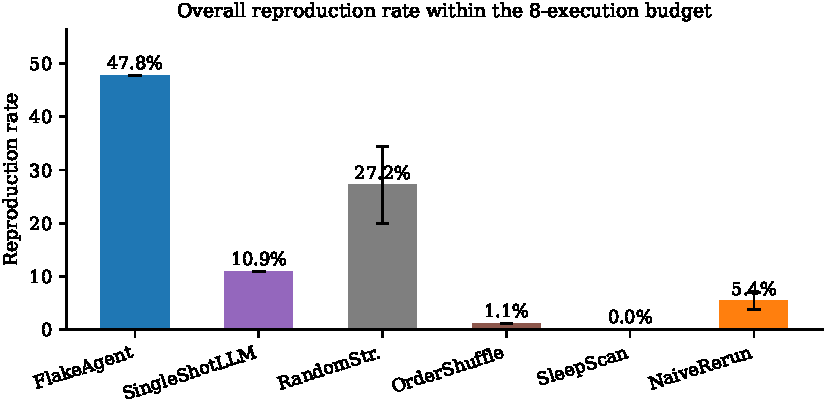
\includegraphics[width=0.92\columnwidth]{figures/repro_overall.pdf}
\caption{Overall reproduction rate: FlakeAgent vs.\ five baselines sharing
the 8-execution budget. Error bars on RandomStrategy, OrderShuffle, and
FlakeAgent are $\pm$ std over 3 seeds on the 30-test variance subset.}
\label{fig:repro-overall}
\end{figure}

\paragraph{Per-category.} Table~\ref{tab:main-results} and
Figure~\ref{fig:repro-category} break reproduction down by category. The
agent's advantage is concentrated where plain rerunning cannot help: it
reproduces every NIO test (via T2) and most ID tests (via T12), categories
where only deliberate execution schemes can expose the failure at all. OD is
the weakest category, as most of its failures trace to cross-class polluters
whose source the agent never sees (Section~\ref{sec:discussion}).

\begin{table}[t]
\caption{Reproduction rates (\% of gate-passed tests) overall and per
category. Best per row in bold, second underlined.}
\label{tab:main-results}
\small
\begin{tabular}{@{}lrrrrrr@{}}
\toprule
 & \textbf{FlakeAgent} & \textbf{NaiveRerun} & \textbf{RandomStr.} &
 \textbf{OrderShuffle} & \textbf{SleepScan} & \textbf{SingleShot}\\
\midrule
Overall & 47.8 & 5.4 & 27.2 & 1.1 & 0.0 & 10.9\\
OD & 20.0 & 0.0 & 15.0 & 5.0 & 0.0 & 5.0\\
TD & 12.9 & 16.1 & 3.2 & 0.0 & 0.0 & 9.7\\
NIO & 100.0 & 0.0 & 84.0 & 0.0 & 0.0 & 24.0\\
ID & 68.8 & 0.0 & 0.0 & 0.0 & 0.0 & 0.0\\
\bottomrule
\end{tabular}
\end{table}

\begin{figure}[t]
\centering
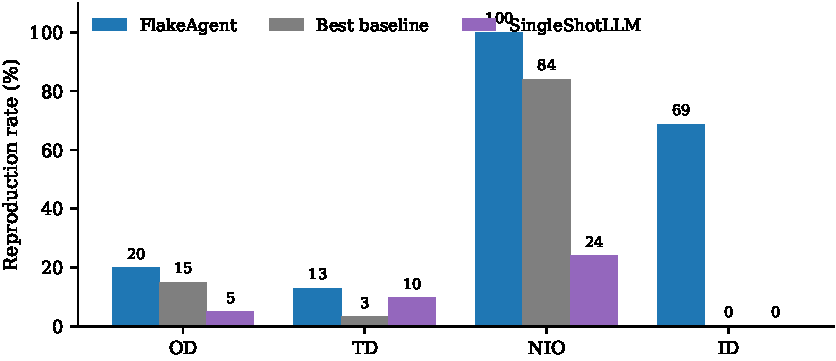
\includegraphics[width=0.92\columnwidth]{figures/repro_category.pdf}
\caption{Reproduction rate by flakiness category (FlakeAgent vs.\ the best
non-agent baseline and SingleShotLLM).}
\label{fig:repro-category}
\end{figure}

\paragraph{Which strategies reproduce what.}
Figure~\ref{fig:heatmap} attributes every reproduction to the triggering
strategy, per ground-truth category. The diagonal is clear: all NIO
reproductions come from T2 (same-JVM double run), most ID from T12 (NonDex),
and OD from T5 (polluter--victim); TD scatters across T1, T10, and T12,
consistent with no single strategy dominating. Two reproductions are T12
fault-injection artifacts whose diagnosed category disagrees with the
ground-truth label (one OD, one TD); we flag them in
Section~\ref{sec:threats} and exclude them from the category-accuracy
discussion below. The heat map is a category $\times$ strategy effectiveness
map, of independent value to practitioners choosing a reproducer.

\begin{figure}[t]
\centering
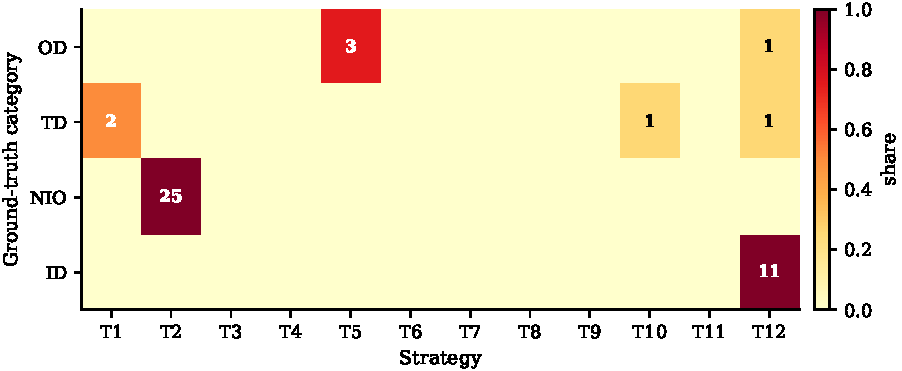
\includegraphics[width=0.95\columnwidth]{figures/heatmap.pdf}
\caption{Category $\times$ strategy reproduction heat map: fraction of
reproductions of each ground-truth category triggered by each strategy
(FlakeAgent runs only).}
\label{fig:heatmap}
\end{figure}

\paragraph{Attempts to reproduction.}
Figure~\ref{fig:atr} (left) shows the ECDF of executions until first
reproduction. FlakeAgent's median ATR is 4.5 executions; 50.0\% of
its reproductions happen within the first 4 executions (i.e., during
or shortly after Step 0 + first planned strategy), and 77.3\% within 5,
with the remainder spread across the loop, evidence of genuine multi-round
search.

\begin{figure}[t]
\centering
\begin{subfigure}[b]{0.48\columnwidth}
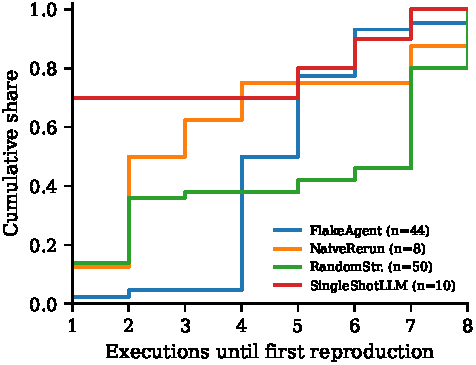
\includegraphics[width=\columnwidth]{figures/atr_ecdf.pdf}
\caption{ECDF of executions until first reproduction.}
\end{subfigure}\hfill
\begin{subfigure}[b]{0.48\columnwidth}
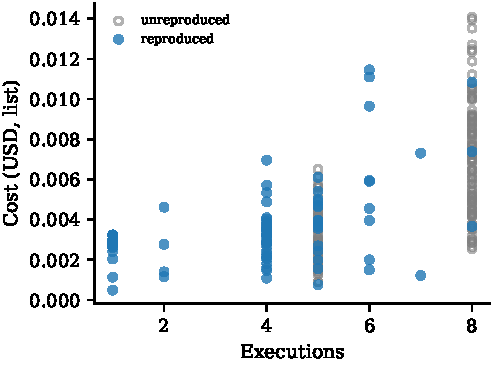
\includegraphics[width=\columnwidth]{figures/cost_scatter.pdf}
\caption{Cost vs.\ attempts per test; reproduced tests in solid, unreproduced
in hollow markers.}
\end{subfigure}
\caption{Search efficiency (left) and cost distribution (right) of
FlakeAgent on the full benchmark.}
\label{fig:atr}
\end{figure}

\subsection{RQ2: Diagnosis accuracy and grounding}
\label{sec:rq2}

On the 44 reproduced tests, the diagnoser commits to a category with
top-1 accuracy 86.4\% exact and 95.5\% coarse (order-dependent vs.\
not). Table~\ref{tab:diagnosis} reports per-category accuracy and, more
importantly, evidence grounding against the developer fix
(\texttt{Fixed.patch}): \emph{evidence precision} is 16.5\% — 17 of 103
cited lines fall inside the fix diff — and \emph{fix-hit} is 36.4\%:
16 of 44 diagnoses cite at least one line the developer changed. The
per-diagnosis \emph{confidence} the model reports correlates moderately with
correctness (Pearson $r = 0.53$; correct diagnoses average 0.86 confidence
vs.\ 0.52 for incorrect ones); we report it but do not rely on it.

\begin{table}[t]
\caption{Diagnosis evaluation on reproduced tests. Evidence is evaluated
against the developer fix diff.}
\label{tab:diagnosis}
\small
\begin{tabular}{@{}lrrrrr@{}}
\toprule
 & \textbf{Diagnosed} & \textbf{Category acc.} & \textbf{Coarse acc.} &
 \textbf{Evid. precision} & \textbf{Fix-hit}\\
\midrule
Overall & 44 & 86.4\% & 95.5\% & 16.5\% & 36.4\%\\
OD & 4 & 50.0\% & 50.0\% & 10.0\% & 25.0\%\\
TD & 4 & 75.0\% & 100.0\% & 10.0\% & 25.0\%\\
NIO & 25 & 100.0\% & 100.0\% & 17.9\% & 40.0\%\\
ID & 11 & 72.7\% & 100.0\% & 18.5\% & 36.4\%\\
\bottomrule
\end{tabular}
\end{table}

\subsection{RQ3: Ablations}
\label{sec:ablation}

Figure~\ref{fig:ablation} and Table~\ref{tab:ablation} report the four
ablations. Removing the reflection loop ($-$reflection) drops reproduction
from 47.8\% to 16.3\% ($-31.5$ pp); shrinking the strategy space ($-$space4)
to 12.0\% and withholding source ($-$source) to 8.0\% on the 50-test subset
(vs.\ 46.0\% for the main config). The gains trace to the reflection loop,
the strategy-space breadth, and source grounding, each contributing
measurably. The Warm configuration isolates the reproduction loop: with the
failure given, the diagnoser commits to a category on 36.0\% of tests (lower
than the 86.4\% cold-start, as a minority of warm replies were unparseable,
Section~\ref{sec:threats}), with evidence grounding comparable to cold-start.

\begin{table}[t]
\caption{Ablations (reproduction \%, diagnosis metrics on each config's own
reproduced subset). $-$reflection runs on the full benchmark; $-$space4,
$-$source, and Warm run on the 50-test stratified subset.}
\label{tab:ablation}
\small
\begin{tabular}{@{}lrrrrr@{}}
\toprule
\textbf{Config} & \textbf{Repro.} & \textbf{Category acc.} &
\textbf{Evid. precision} & \textbf{Fix-hit} & \textbf{\$/test}\\
\midrule
FlakeAgent (main) & 47.8\% & 86.4\% & 16.5\% & 36.4\% & 0.0066\\
$-$reflection & 16.3\% & 80.0\% & 16.1\% & 26.7\% & 0.0032\\
$-$space4 & 12.0\% & 83.3\% & 25.0\% & 50.0\% & 0.0075\\
$-$source & 8.0\% & 100.0\% & 11.1\% & 25.0\% & 0.0053\\
Warm & n/a & 36.0\% & 16.0\% & 12.0\% & 0.0024\\
\bottomrule
\end{tabular}
\end{table}

\begin{figure}[t]
\centering
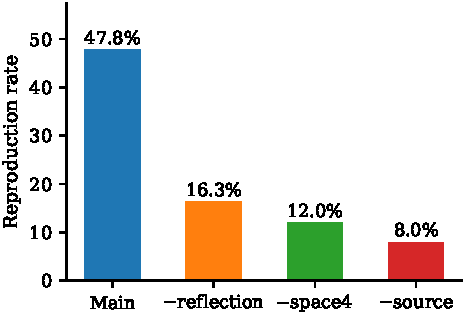
\includegraphics[width=0.92\columnwidth]{figures/ablation.pdf}
\caption{Ablation results: reproduction rate for the four ablations vs.\
the main configuration.}
\label{fig:ablation}
\end{figure}

\subsection{RQ4: Cost}
\label{sec:cost}

Table~\ref{tab:cost} and Figure~\ref{fig:atr} (right) report the cost
profile. At \$0.006 USD median per test (list prices), reproducing one flaky
failure costs \$0.014 USD on average; the distribution is right-skewed
(median \$0.0066, p90 \$0.01) because the loop is budget-bounded rather than
cost-bounded, and wall-clock follows the same pattern (median 1.55 min, p90
3.71 min). The whole 92-test benchmark costs \$0.60 USD in total. By
comparison, the dataset's own validation gate runs up to 10 official-mechanism
invocations per test, each an order of magnitude slower than one agent
execution; FlakeAgent reproduces the same failures at under a cent per test,
and adds a diagnosis no rerun loop can provide.

\begin{table}[t]
\caption{Cost profile of FlakeAgent (main configuration, full benchmark, at
provider list prices; usage from provider-reported metadata).}
\label{tab:cost}
\small
\begin{tabular}{@{}lrrrr@{}}
\toprule
\textbf{Metric} & \textbf{Median} & \textbf{Mean} & \textbf{p90} & \textbf{Total}\\
\midrule
LLM calls per test & 5.0 & 3.95 & 5.0 & 363\\
Executions per test & 8.0 & 6.43 & 8.0 & 592\\
Input tokens per test & 13{,}833 & 14{,}434 & 27{,}376 & 1{,}327{,}944\\
Output tokens per test & 5{,}932 & 7{,}336 & 13{,}605 & 674{,}927\\
Cost per test (USD) & 0.006 & 0.0066 & 0.01 & 0.60\\
Cost per reproduction (USD) & \multicolumn{3}{c}{--} & 0.014\\
Wall-clock per test (min) & 1.55 & 2.36 & 3.71 & 216\\
\bottomrule
\end{tabular}
\end{table}

\subsection{Cross-model comparison}

Table~\ref{tab:models-results} compares the six models on the stratified
50-test subset under the identical protocol (same prompts, budgets,
temperature; only the model differs). DeepSeek-V4.1-Flash reproduces 46.0\%,
while the other five cluster tightly at 10--12\%. The gap between the best
and worst model (46.0\% vs.\ 10.0\%, 36~pp) is comparable to the gap between
FlakeAgent and its ablations ($-$source 8.0\%), so model choice matters as
much as design choice on this task. The frontier reasoning-heavy models do
not outperform their cheaper sibling here: at low reasoning effort their
visible reply is small and their plan quality suffers
(Section~\ref{sec:setup}). DeepSeek-V4.1-Flash's edge is likely both a
stronger prior and the 4{,}000-token output budget that lets its reasoning
survive the visible-reply cap.

\begin{table}[t]
\caption{Cross-model comparison on the 50-test stratified subset
(reproduction \%, diagnosis, cost per test at list prices).}
\label{tab:models-results}
\small
\begin{tabular}{@{}lrrrrr@{}}
\toprule
\textbf{Model} & \textbf{Repro.} & \textbf{Category acc.} &
\textbf{Evid. precision} & \textbf{Fix-hit} & \textbf{\$/test}\\
\midrule
DeepSeek-V4.1-Flash & 46.0\% & 82.6\% & 18.2\% & 39.1\% & 0.0066\\
DeepSeek-V4-Pro & 12.0\% & 83.3\% & 14.3\% & 16.7\% & 0.0353\\
Gemini-3.8-Flash & 10.0\% & 80.0\% & 28.6\% & 40.0\% & 0.0070\\
Grok-4.7 & 12.0\% & 66.7\% & 12.5\% & 16.7\% & 0.0300\\
GPT-5.6 & 12.0\% & 100.0\% & 0.0\% & 0.0\% & 0.0374\\
GPT-6-Astra & 10.0\% & 100.0\% & 10.0\% & 20.0\% & 0.0928\\
\bottomrule
\end{tabular}
\end{table}

\subsection{Reliability}

On the 30-test variance subset, FlakeAgent's mean reproduction rate across 3
seeds is 28.9 $\pm$ 8.4\% (RandomStrategy: 15.6 $\pm$ 10.2\%, NaiveRerun:
5.6 $\pm$ 1.6\%). The agent's variance is larger than the baselines', which
is expected: its decisions are sampled from an LLM planner, so early-round
strategy choices diverge across seeds; we flag this sampling noise in
Section~\ref{sec:threats}.
